\documentclass[export,border=0pt]{standalone}
\usepackage[T1]{fontenc}
\usepackage{amsmath,amsfonts}
\usepackage{grid-guide}
\usepackage{tikz}
\usetikzlibrary{shapes.geometric} % Cylinder
\usetikzlibrary{shadows.blur,arrows.meta,bending,positioning}
\usetikzlibrary{%
	calc,%
	decorations.pathmorphing,%
	fadings,%
	shadings,
   decorations.pathreplacing,calligraphy
}
\usepackage{animate}

\begin{document}
\begin{animateinline}[loop]{90}
    \multiframe{90}{i=0+1}{
  \begin{tikzpicture}[remember picture]
    \node[anchor=center,opacity=0.5](i1) at (10,3.5){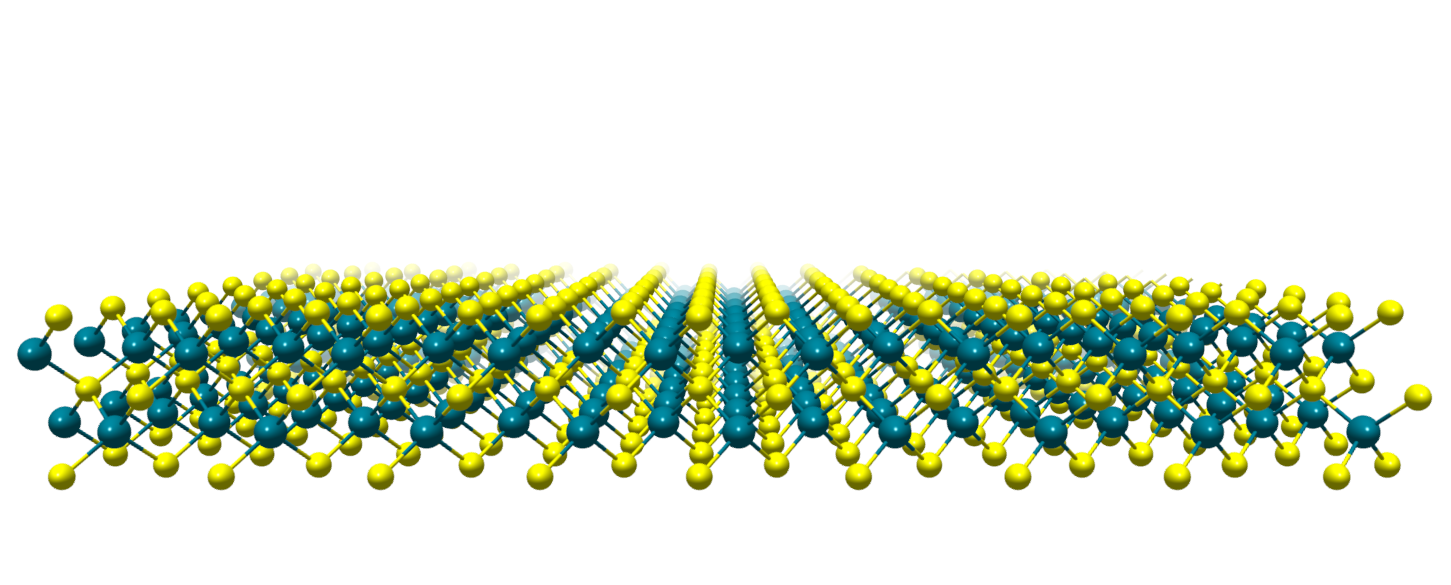
\includegraphics[width=\paperwidth]{atom-line.png}};
    %  \draw[labeled grid](0,0) to (20,7);   
    \begin{scope}[yshift=2cm,xshift=1cm]
        \def\x{\i}
        \def\xmax{\i}
        \pgfmathsetmacro\xx{\i*0.2};
        \draw[variable=\xx,smooth,domain=0:\xx,color=red]plot[mark=*,mark options={scale=1.5},line width=2pt](\xx,{2*sin(50*\xx)});
    \end{scope}
        
   \node[red, scale=3,anchor=north west] at (i1.north west){$\psi(r)=e^{ik\cdot r}u(r)$};
  \end{tikzpicture}
  }
\end{animateinline}
\end{document} 
% \draw[ultra thick, red] (0,2) sin (3,4)cos(6,2) sin (9,0) cos(12,2)sin (15,4)cos (18,2);
